\documentclass{article}
\usepackage[a4paper, margin=2.5cm]{geometry}
\usepackage{polski, graphicx, float, hyperref}
\setcounter{secnumdepth}{0}

\begin{document}
\subsection{Podział architektury systemu}
System integracji drona Geopixel Sharky jest podzielony na 2 główne części:
\begin{itemize}
    \item Dodanie aparatury 5G na pokładzie drona
    \item Stworzenie stacji naziemnej do obsługi drona
\end{itemize}

\subsection{Aparatura 5G na pokładzie drona}
\subsubsection{Wykorzystany sprzęt}

\begin{itemize}
    \item Modem 5G - RM500x / RM502x 5G HAT
    \item Raspberry Pi 4
    \item Kamera ip - ms-c9674-pa
\end{itemize}

\subsubsection{Schemat blokowy}
Kolorem niebieskim zaznaczono elementy, które są dokładne do drona w ramach projektu\\
Kolorem zielonynm zaznaczono elementy, które są już obecne.

\begin{figure}[H]
    \centering
    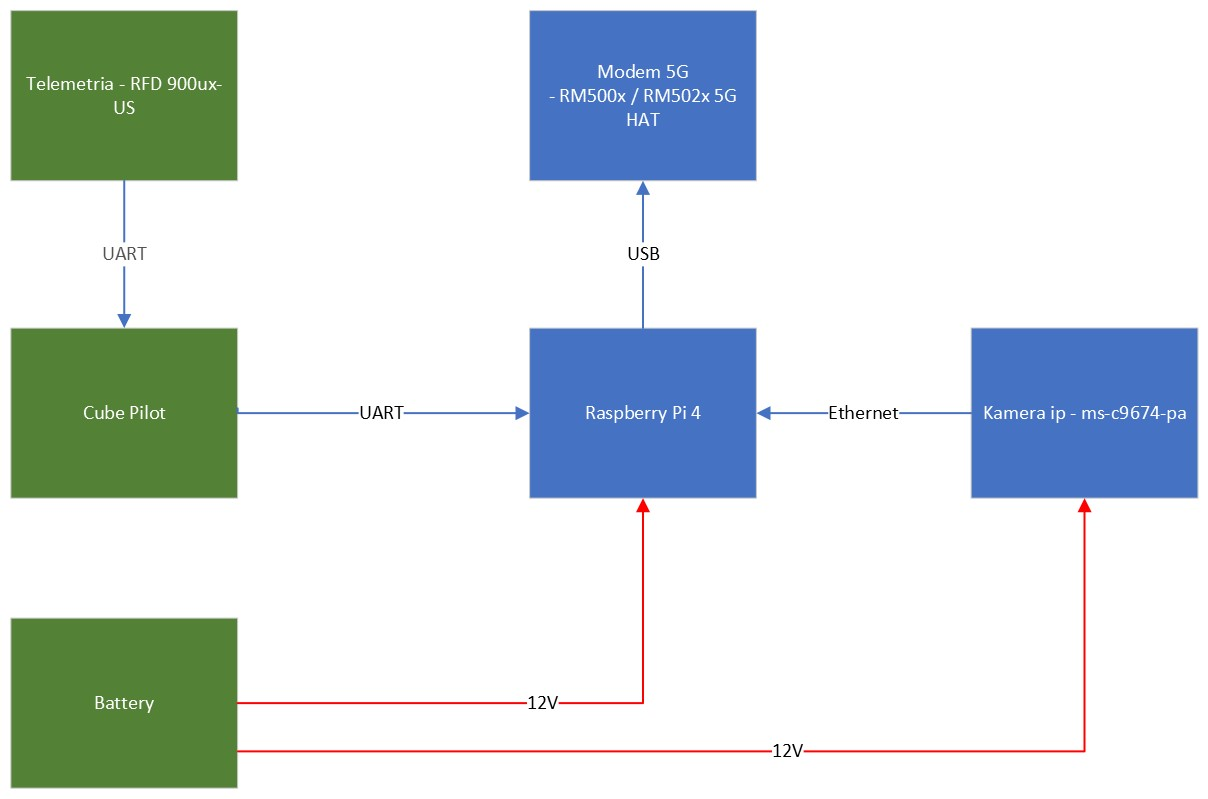
\includegraphics[width=0.9\textwidth]{nadronie.jpg}
    \caption{Schemat blokowy modułu}
\end{figure}

\subsubsection{Opis działania}
Na dronie obecnie się znajduje moduł Cube pilot na którym działa oprogramowanie ardupilot. Oprogramowanie to realizuje telemetrię w oparciu o protokół MAVlink.
Obecnie łącze telemetryczne w warstwie sprzętowej wykorzystuje port szeregowy Cube pilota do którego podłączony jest moduł radiowy. Wykorzystując oprogramowanie 
MAVproxy działające na Rassbery pi możemy wysyłać oraz odbierać protokół MAVlink enkapsulowany w protokole UDP co pozwala nam ustanowić połczenie MAVlink poprzez sieć 5G.
MAVproxy umożliwia utworzenie mostu pomiędzy łączem MAVlink opartym o port szeregowy a łączem opartym o protokół IP. Dane z kamery połączonej do Rassbery pi poprzez ethernet 
wysyłane są przez sieć 5G poprzez porgramowy most pomiędzy fizycznym portem ethernet a wirtualnym portem ethernet używanym przez modem 5G.


\subsubsection{Problemy do rozwiązania}
Znaleźć rozwiązanie programowe pozwalające zmostkować strumień obrazu z kamery IP z interfejsu ethernet Rassbery Pi do modemu 5G.
Sparawdzić czy układy nie wymagają dołożenia odzielnego zasilacza z wyższą wydajnością prądową.

\subsection{Stacja naziemna}
\subsubsection{Wykorzystany sprzęt}
\begin{itemize}
    \item Bramka 5G
    \item Komputer przemysłowy
    \item Joystick
    \item Monitor
    \item Przełącznik uzbrojenia
    \item Zasilacz
\end{itemize}

\subsubsection{Schemat blokowy}

\begin{figure}[H]
    \centering
    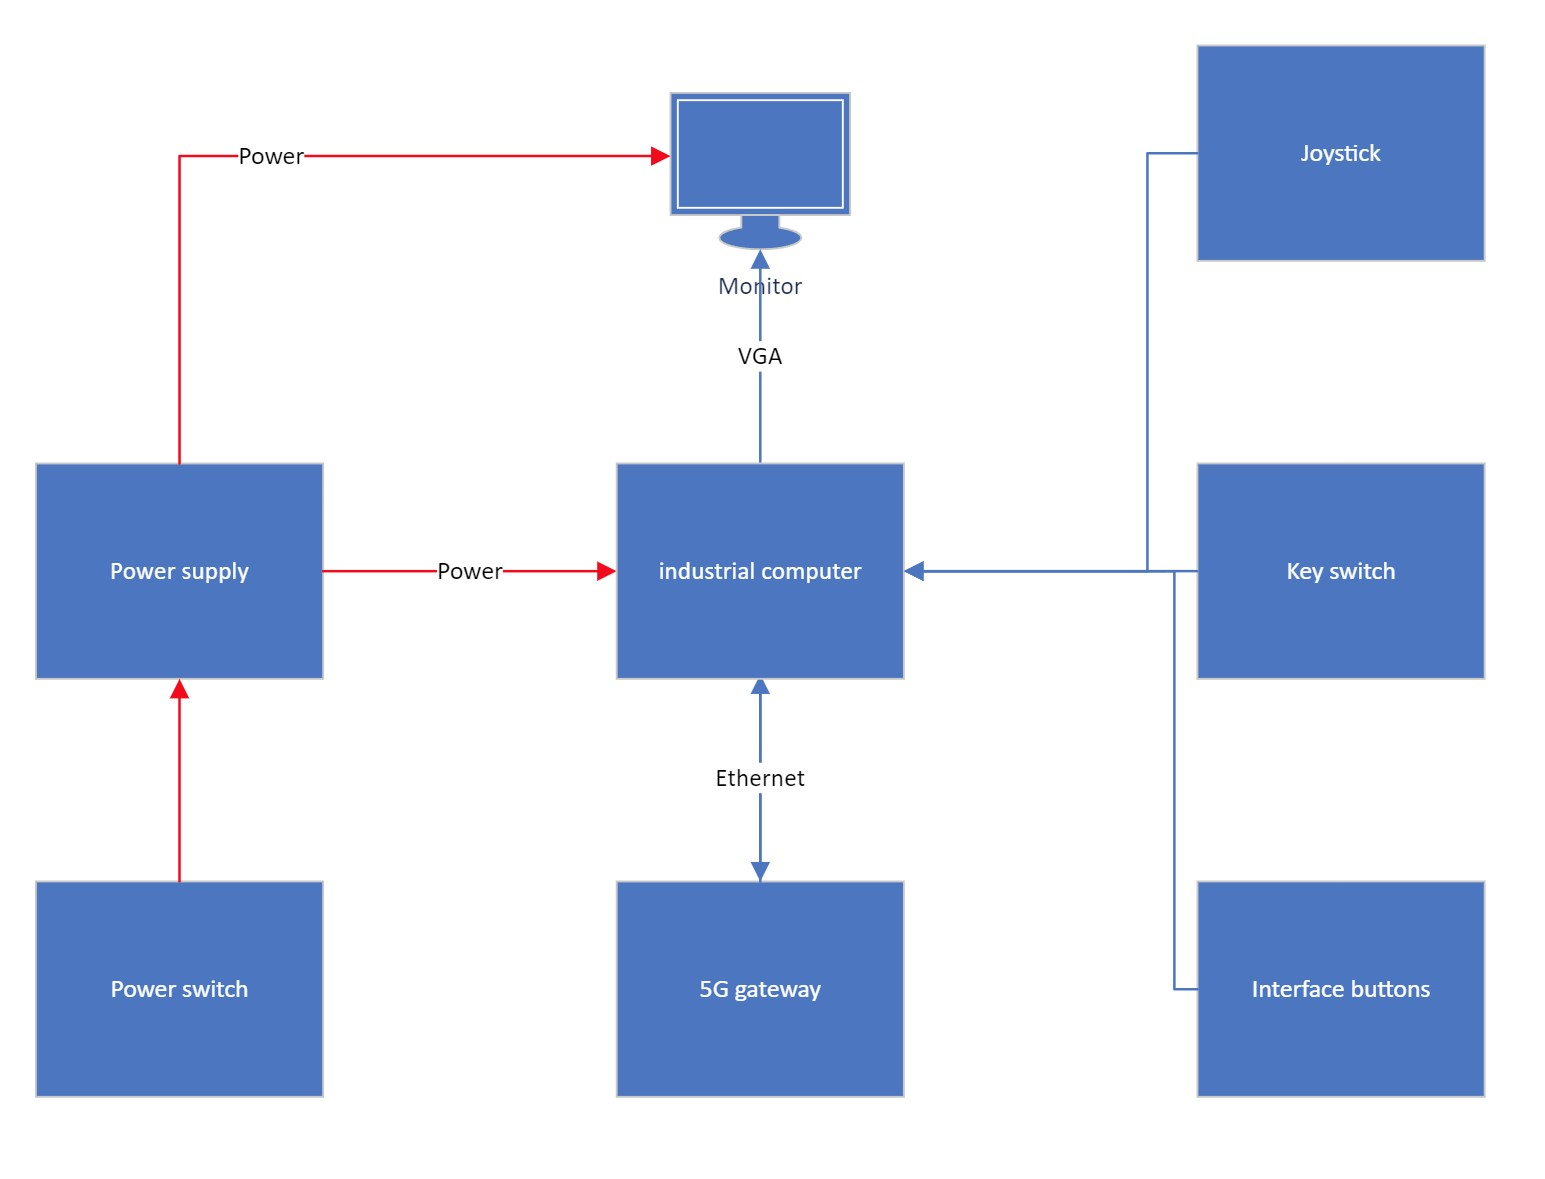
\includegraphics[width=0.9\textwidth]{stacja.jpg}
    \caption{Schemat blokowy stacji naziemnej}
\end{figure}

\subsubsection{Opis działania}
Stacja ma zadanie służyć za interfejs użytkownika do sterowania dronem.
Ma za zadanie odbierać dane z drona i wyświetlać je na monitorze oraz przekazywać na pojazd dane kontrolne oraz sygnały sterujące.
Sercem stacji będzie komputer przemysłowy z systemem linux, który będzie posiadał połączenie do bramki 5G co umożliwi mu komunikacje z pojazdem. 
QGroundControl który jest dedykowanym oprogramowaniem stacjinaziemnej dla pojazdów opierających swoją telemetrie o protokół MAVlink. Możliwe jest również zastosowanie dodatkowe mikrokontrolera do komunikacji z peryferiami, takimi jak joysticki, przyciski, przełączniki, któty będzie się komunikował z 
komputerem przemysłowym za pomocą portu szeregowego.

\subsubsection{Problemy do rozwiązania}
Na obecnym etapie trzeba dobrać konkretne komopotenty, które będą spełniały wymagania projektu.

\end{document}
